\documentclass{article}

\usepackage{times}
\usepackage{geometry}
\geometry{a4paper,left=0.6cm,right=0.7cm,top=2cm,bottom=1cm,columnsep=0.8cm}
\usepackage{fontawesome}
\usepackage[hidelinks]{hyperref}
\usepackage{multicol}
\usepackage{tikz}
\usepackage{hyphsubst}
\usepackage{moresize}
\usepackage{hyphenat}
\usepackage{tabularx}
\usepackage{xcolor}
\usepackage{enumitem}
\usetikzlibrary{calc, positioning}      
\newcolumntype{Y}{>{\RaggedRight\arraybackslash}X}

% Définition des couleurs
\definecolor{maincolor}{HTML}{f0fafc}
\definecolor{seccolor}{HTML}{ffffff}
\definecolor{gray}{HTML}{8c94a9}
\definecolor{sidetext}{HTML}{59cee5}

% Solution robuste pour la bande bleue sur toute la hauteur
\usepackage{eso-pic}
\AddToShipoutPictureBG{%
  \begin{tikzpicture}[remember picture,overlay]
    \fill[maincolor] 
        (current page.north west) rectangle 
        ([xshift=0.3\paperwidth] current page.south west);
  \end{tikzpicture}%
}

% Configuration des listes
\setlist[itemize]{itemsep=-2pt,topsep=0pt,leftmargin=1.08cm}
\renewcommand{\labelitemi}{\textcolor{sidetext}{\footnotesize$\bullet$}}

\setlength{\parindent}{0pt}
\usepackage{paracol}
\columnratio{0.3}

\begin{document}

\pagestyle{empty}

\begin{paracol}{2}
% Colonne gauche - Section personnelle
\color{sidetext}
\begin{center}
    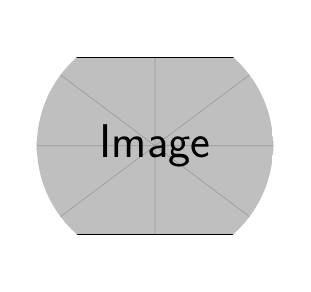
\begin{tikzpicture}
        \clip (0,0) circle (1.5cm) node[anchor=center] {\includegraphics[width=3cm]{example-image}}; 
    \end{tikzpicture}

    \vspace{5mm}
    
    {\color{black}\LARGE \textbf{Jean Dupont}}
    
    \vspace{3mm}
    
    {\large{Ingénieur Logiciel Senior}}
\end{center}

{\color{gray}\rule{\linewidth}{0.4pt}} \\

% Coordonnées
\begin{tabular}{@{}c l}
    \faPhone & 
    \begin{tabular}[t]{@{}l@{}}
        {\color{gray}Téléphone} \\
        06 12 34 56 78
    \end{tabular} \\
    \\
    \faLinkedin & 
    \begin{tabular}[t]{@{}l@{}}
        {\color{gray}LinkedIn} \\
        \href{https://linkedin.com/in/jeandupont}{linkedin.com/in/jeandupont}
    \end{tabular} \\
    \\
    \faMapMarker & 
    \begin{tabular}[t]{@{}l@{}}
        {\color{gray}Adresse} \\
        123 Rue de Paris, 75001 Paris
    \end{tabular} \\
    \\
    \faEnvelope & 
    \begin{tabular}[t]{@{}l@{}}
        {\color{gray}Email} \\
        \href{mailto:jean.dupont@email.com}{jean.dupont@email.com}
    \end{tabular} \\
\end{tabular}

\vspace{3mm}
{\color{gray}\rule{\linewidth}{0.4pt}} \\

% Langues
{\color{black}{Langues}}

\vspace{3mm}

\begin{tabular}{@{}c l}
    \faLanguage & 
    \begin{tabular}[t]{@{}l@{}}
        Français \\
        {\color{gray}{Langue maternelle}} \\
        \\
        Anglais \\
        {\color{gray}{Courant}} \\
        \\
        Espagnol \\
        {\color{gray}{Intermédiaire}}
    \end{tabular} \\
\end{tabular}

\vspace{5mm}
{\color{gray}\rule{\linewidth}{0.4pt}} \\

% Compétences - CORRECTION DES ICÔNES ICI (utiliser uniquement des icônes standard)
\vspace{5mm}
{\color{black}{Compétences Clés}}

\vspace{5mm}

\begin{tabular}{@{}c l}
    \textcolor{sidetext}{\faCode} & Développement Web (HTML/CSS/JS) \\
    \\
    \textcolor{sidetext}{\faDatabase} & Bases de données (SQL, NoSQL) \\
    \\
    \textcolor{sidetext}{\faServer} & Architecture Cloud (AWS, Azure) \\
    \\
    \textcolor{sidetext}{\faGit} & Git \& Méthodes Agile \\
    \\
    \textcolor{sidetext}{\faUsers} & Gestion d'équipe \\
    \\
    % Icône standard pour Négociation commerciale
    \textcolor{sidetext}{\faComments} & Négociation commerciale \\
    \\
    % Icône standard pour Organisation
    \textcolor{sidetext}{\faCalendar} & Organisation \\
    \\
    % Icône standard pour Relations
    \textcolor{sidetext}{\faGroup} & Relations \\
\end{tabular}

% Espace flexible pour étendre la colonne gauche
\vfill
~

\switchcolumn
% Colonne droite - Contenu professionnel
\color{black}

% Résumé professionnel
\textcolor{black}{\Large \textbf{Profil Professionnel}} \\

\textcolor{black}{Ingénieur logiciel avec 10 ans d'expérience dans le développement d'applications web et mobiles. Expertise en architecture de systèmes distribués et en gestion de projets complexes. Passionné par les technologies émergentes et les méthodes de développement agile.}\\[8pt]

% Expérience professionnelle
\textcolor{black}{\Large \textbf{Expérience Professionnelle}} \\

% Expérience 1
\colorbox{maincolor}{%
  \begin{minipage}{\linewidth}
    \begin{tabular}{@{}l l r}
        \textcolor{sidetext}{\faBriefcase} & 
        \textbf{Senior Tech Lead} &  
        \footnotesize{2020 - Présent} \\
        & \textit{Innovatech Solutions} & \\
    \end{tabular}
    \begin{itemize}
        \item Direction d'une équipe de 10 développeurs sur des projets cloud
        \item Conception d'architecture microservices pour applications critiques
        \item Mise en place de pipelines CI/CD et d'infrastructure IaC
    \end{itemize}
  \end{minipage}%
}

\vspace{5mm}

% Expérience 2
\colorbox{maincolor}{%
  \begin{minipage}{\linewidth}
    \begin{tabular}{@{}l l r}
        \textcolor{sidetext}{\faBriefcase} & 
        \textbf{Développeur Full Stack} &  
        \footnotesize{2015 - 2020} \\
        & \textit{WebCréation} & \\
    \end{tabular}
    \begin{itemize}
        \item Développement d'applications web avec React et Node.js
        \item Optimisation des performances et expérience utilisateur
        \item Intégration de solutions de paiement et d'API tierces
    \end{itemize}
  \end{minipage}%
}

\vspace{8mm}

% Formation
\textcolor{black}{\Large \textbf{Formation}} \\

% Diplôme 1
\begin{tabular}{@{}c l}
    \textcolor{sidetext}{\faGraduationCap} & 
    \begin{tabular}[t]{@{}l@{}}
        \textbf{Master en Informatique} \\
        Université Paris-Saclay \\
        Spécialisation: Architecture Logicielle \\
        2012 - 2015
    \end{tabular} \\
\end{tabular}

\vspace{5mm}

% Diplôme 2
\begin{tabular}{@{}c l}
    \textcolor{sidetext}{\faGraduationCap} & 
    \begin{tabular}[t]{@{}l@{}}
        \textbf{Licence en Informatique} \\
        Université Paris Descartes \\
        Mention Très Bien \\
        2009 - 2012
    \end{tabular} \\
\end{tabular}



\end{paracol}

\end{document}